\chapter{Razvojni sustav ESP32-C3-DevKitM-1}

Razvojni sustav temelji se na modulu ESP32-C3-MINI-1. Modul je jedan u nizu ESP32-­C3 serije SoC (engl. \textit{System on Chip}) platformi tvrtke \textit{Espressif}, te sadrži jednojezgreni 32-bitni procesor s RISC-V arhitekturom koji radi na frekvenciji do 160 MHz. Modul sadrži 400 KB memorije tipa SRAM (engl. \textit{Static random-access memory}), od kojih je 16 KB rezervirano za priručnu memoriju (engl. \textit{cache}), 384 MB memorije tipa ROM (engl. \textit{Read-only memory}) te 4 MB memorije tipa \textit{Flash}. Od periferije sadrži 22 programabilna GPIO pina (engl. \textit{General Purpose Input Output}), te digitalna sučelja SPI, UART, I2C i I2S. Također sadrži upravljače za sučelja USB i JTAG koji se mogu koristiti za efikasnije otklanjanje pogrešaka u kodu (engl. \textit{debugging}). Konfiguracija sustava prikazana je na slici \ref{fig:esp32}. \cite{esp32manual}

\begin{figure}[ht]
	\centering
	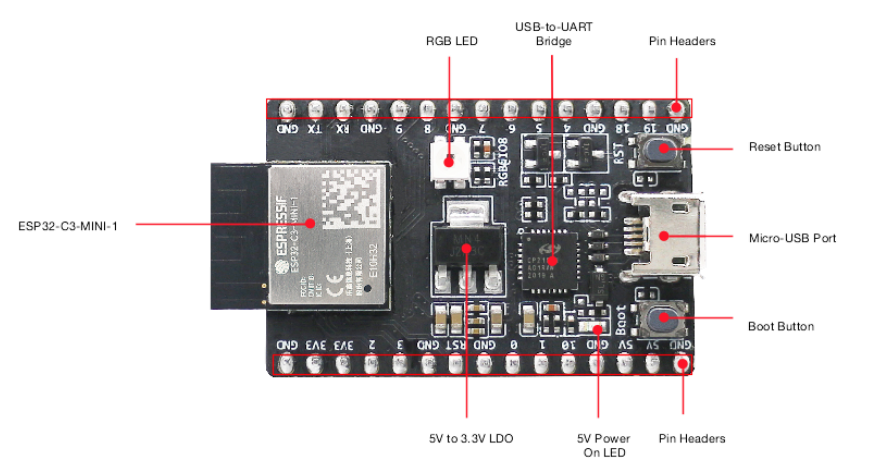
\includegraphics[scale=0.6]{imgs/esp32}
	\caption{Konfiguracija razvojnog sustava ESP32-C3-DevKitM-1 \cite{espressif}}
	\label{fig:esp32}
\end{figure}

Budući da modul ima funkciju RF (engl. \textit{radio frequency}) primopredajnika, podržava bežično lokalno umrežavanje odnosno Wi-Fi, koji omogućava propusnost do 20 Mbps protokolom TCP te maksimalnu propusnost od 30 Mbps koristeći protokol UDP. Isto tako, podržava protokol Bluetooth s podrškom za velike udaljenosti. 

Modul ESP32-C3-MINI-1 bežični je uređaj niske potrošnje energije (engl. \textit{ultra-low-power}) primarno namijenjen razvoju aplikacija koje koriste Wi-Fi ili \textit{Bluetooth Low Energy} (BLE) protokol. Na slici \ref{fig:esp32block} nalazi se blok shema modula sa svim dostupnim značajkama. 

\begin{figure}[ht]
	\centering
	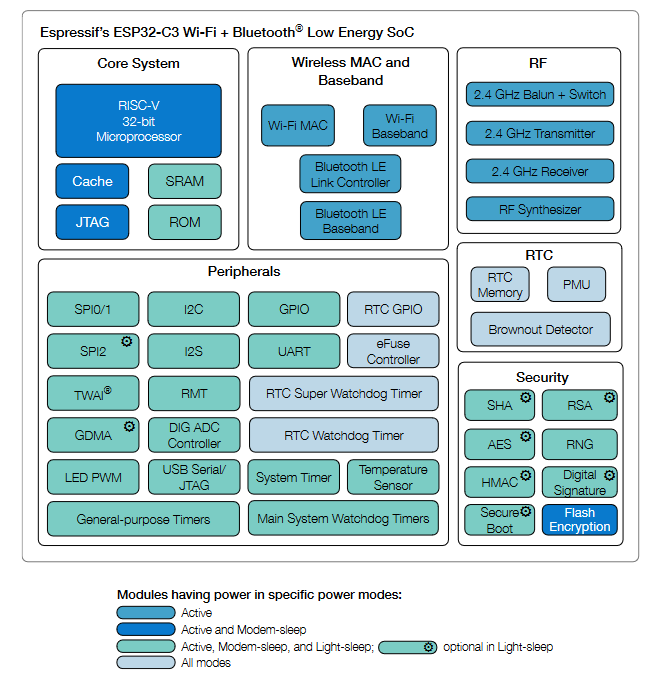
\includegraphics[scale=0.6]{imgs/esp32block}
	\caption{Blok dijagram modula ESP32-C3 \cite{esp32manual}}
	\label{fig:esp32block}
\end{figure}

\section{Wi-Fi}

IEEE 802.11, skupina standarda za bežične lokalne mreže (engl. \textit{WLANs}) \cite{ieee}, nudi nekoliko različitih načina bežične modulacije signala. Pojedini standardi označeni su slovima abecede. Za korisničke mreže postoje dva frekvencijska pojasa: 2,4 GHz i 5 GHz. 

Prednosti pojasa od 2,4 GHz su veći doseg, bolje prolaženje kroz fizičke prepreke te bolja podrška jer više bežičnih uređaja koristi pojas od 2,4 GHz nego od 5 GHz. S druge strane, ovaj pojas ima manju propusnost i nudi manje kanala koji se ne preklapaju. Isto tako, može doći do zagušenja mreže jer kućni i Bluetooth uređaji koriste ovaj isti mrežni pojas.

Pojas od 5 GHz nudi brži protok, manje zagušenih kanala te ima više kanala koji se međusobno ne preklapaju. Ipak, ima kraći raspon u usporedbi s mrežama od 2,4 GHz jer teže prolazi kroz prepreke. \cite{microsoft_ieee} 

U nastavku su opisani ključni standardi Wi-Fi tehnologije \cite{how_wifi_works}:
\begin{itemize}
	\item 802.11b - najsporiji i najjeftiniji standard, emitira u frekvencijskom pojasu od 2,4 GHz. Može prenijeti do 11 Mbps te koristi komplementarno šifriranje (engl. \textit{complementary code keying - CCK}) radi poboljšanja brzine prijenosa.
	\item 802.11a - transmitira u pojasu od 5 GHz i može prenijeti do 54 Mbps. Koristi ortogonalno frekvencijsko multipleksiranje (engl. \textit{orthogonal frequency-division multiplexing - OFDM}), što je efikasnija tehnika u odnosu na CCK koja dijeli radio signal u nekoliko podsignala prije slanja primatelju. Ova metoda značajno umanjuje interferenciju. 
	\item 802.11g - poput standarda 802.11b, koristi frekvencijski pojas od 2,4 GHz. Međutim, može prenijeti do 54 Mbps jer koristi tehniku OFDM.
	\item 802.11n - kompatibilan je standard sa prethodno opisanim standardima. Nudi znatno poboljšanje u rasponu i brzini u odnosu na svoje prethodnike. Ovaj standard može prenijeti do četiri toka podataka, svaki maksimalno 150 Mbps, no većina usmjerivača (engl. \textit{router}) dopušta dva ili tri toka.
	\item 802.11ac - radi isključivo u pojasu od 5 GHz, te je kompatibilan s prethodnim standardima. Manje je sklon interferenciji i brži je od prethodnih standarda s maksimalnim prijenosom od 450 Mbps jednim tokom. 
	\item 802.11ax - najnoviji standard koji proširuje nekoliko ključnih mogućnosti svojih prethodnika. Usmjerivači koji podržavaju ovaj standard dopuštaju tok podataka do 9.2 Gbps, što je značajan porast u usporedbi s prethodnicima. Isto tako, moguće je postaviti više antena na jedan usmjerivač, čime je omogućen prihvat više veza odjednom bez usporavanja i interferencije.
\end{itemize}

Podsustav modula ESP32-C3 za Wi-Fi u skladu je sa standardom IEEE 802.111 te koristi nelicencirani pojas frekvencija od 2,4 GHz. U tom pojasu podržava propusnost od 20 i 40 MHz. Modul također podržava tehniku raznolikosti antena (engl. \textit{antenna diversity}) za poboljšanje prijema i pouzdanosti signala korištenjem RF komutatora (engl. \textit{switch}). Tim komutatorom upravljaju GPIO priključci i koristi se za odabir najbolje antene u kontekstu pouzdanosti i kvalitete signala. \cite{esp_mini}

ESP32-C3 u potpunosti implementira protokol Wi-Fi na temelju standarda 802.11 b/g/n. Podržava osnovni skup (engl. \textit{Basic Service Set - BSS}) operacija za značajke pristupne točke (engl. \textit{SoftAP}). Upravljanje napajanjem odvija se automatski s minimalnom intervencijom domaćina kako bi se smanjila aktivnost uređaja.

Tvrtka \textit{Espressif} također nudi biblioteke za povezivanje putem protokola TCP i IP te korištenje Wi-Fi \textit{mesh} tehnologije. Pruža i podršku za protokole TLS 1.0, 1.1 i 1.2. Na slici \ref{fig:wifi_rf_table} prikazani su Wi-Fi RF standardi koje koristi modul. 

\begin{figure}[ht]
	\centering
	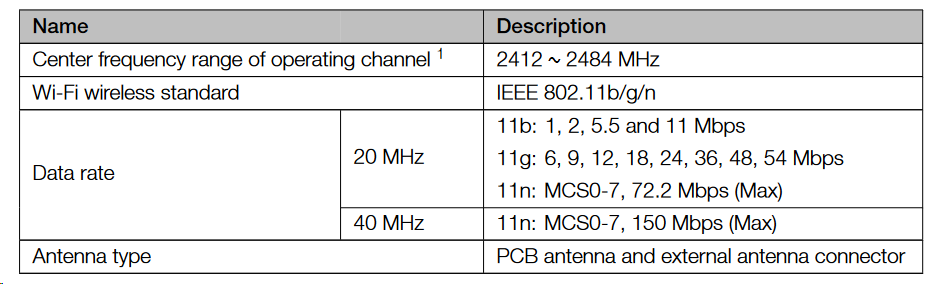
\includegraphics[scale=0.5]{imgs/wifi_rf_table}
	\caption{Wi-Fi RF standardi \cite{esp_mini}}
	\label{fig:wifi_rf_table}
\end{figure}

ESP32 nudi nekoliko načina rada pri korištenju Wi-Fi tehnologije \cite{esp_wifi_connect_overview}:
\begin{enumerate}
	\item način rada stanice (engl. \textit{station mode}) - ESP32 spaja se na točku pristupa,
	\item način rada pristupne točke (engl. \textit{SoftAP mode}) - druge se stanice spajaju na ESP32,
	\item miješani - ESP32 radi kao stanica i pristupna točka spojena na drugu pristupnu točku. 
\end{enumerate}

U nastavku su opisani scenariji Wi-Fi povezivanja modula ESP32-C3 u načinu rada stanice i pristupne točke.

Na slici \ref{fig:station_scenario} prikazan je sekvencijski dijagram zadataka koje ESP32 obavlja u cijelom ciklusu spajanja i komunikacije s pristupnom točkom. Iz slike je vidljivo da se ciklus sastoji od osam faza. Prva faza služi za inicijalizaciju upravljačkih programa i pokretanje zadataka odnosno dretvi koje će obavljati zadatke vezane uz svoju dužnost. Glavni zadatak pokreće četiri različite dretve izvršavanja: aplikacijski zadatak, zadatak za događaje, zadatak za IP protokol, te zadatak za Wi-Fi. U drugoj fazi konfigurira se upravljački program za Wi-Fi. U sljedećoj se fazi pokreće upravljački program, nakon koje slijedi faza pretraživanja mreže i povezivanja na usmjerivač ili pristupnu točku. Nakon inicijalizacije DHCP klijenta, započinje faza dohvata IP adrese. Šesta faza odvija se nakon prekida Wi-Fi veze, čime se također uklanjaju i sve UDP i TCP konekcije. U aplikaciji se može omogućiti radno čekanje na ponovno uspostavljanje veze. Sedma faza pokreće se pri detekciji promjene IP adrese. Posljednja faza služi za programsko odspajanje s mreže i zaustavljanje upravljačkog programa za Wi-Fi.

Slika \ref{fig:ap_scenario} modelira slučaj u kojem ESP32 ima ulogu pristupne točke. Scenarij je vrlo sličan ranije opisanom slijedu događaja, no razlikuje se u dvije faze i događajima koji su pohranjeni u sustavu. Ovaj način rada nema fazu detekcije promjene IP adrese, jer je u ovom načinu ESP32 upravo taj uređaj čija se IP adresa može promijeniti. Isto tako, ne postoji faza dohvata IP adrese. 

\begin{figure}[ht]
	\begin{minipage}[t]{0.4\textwidth}
		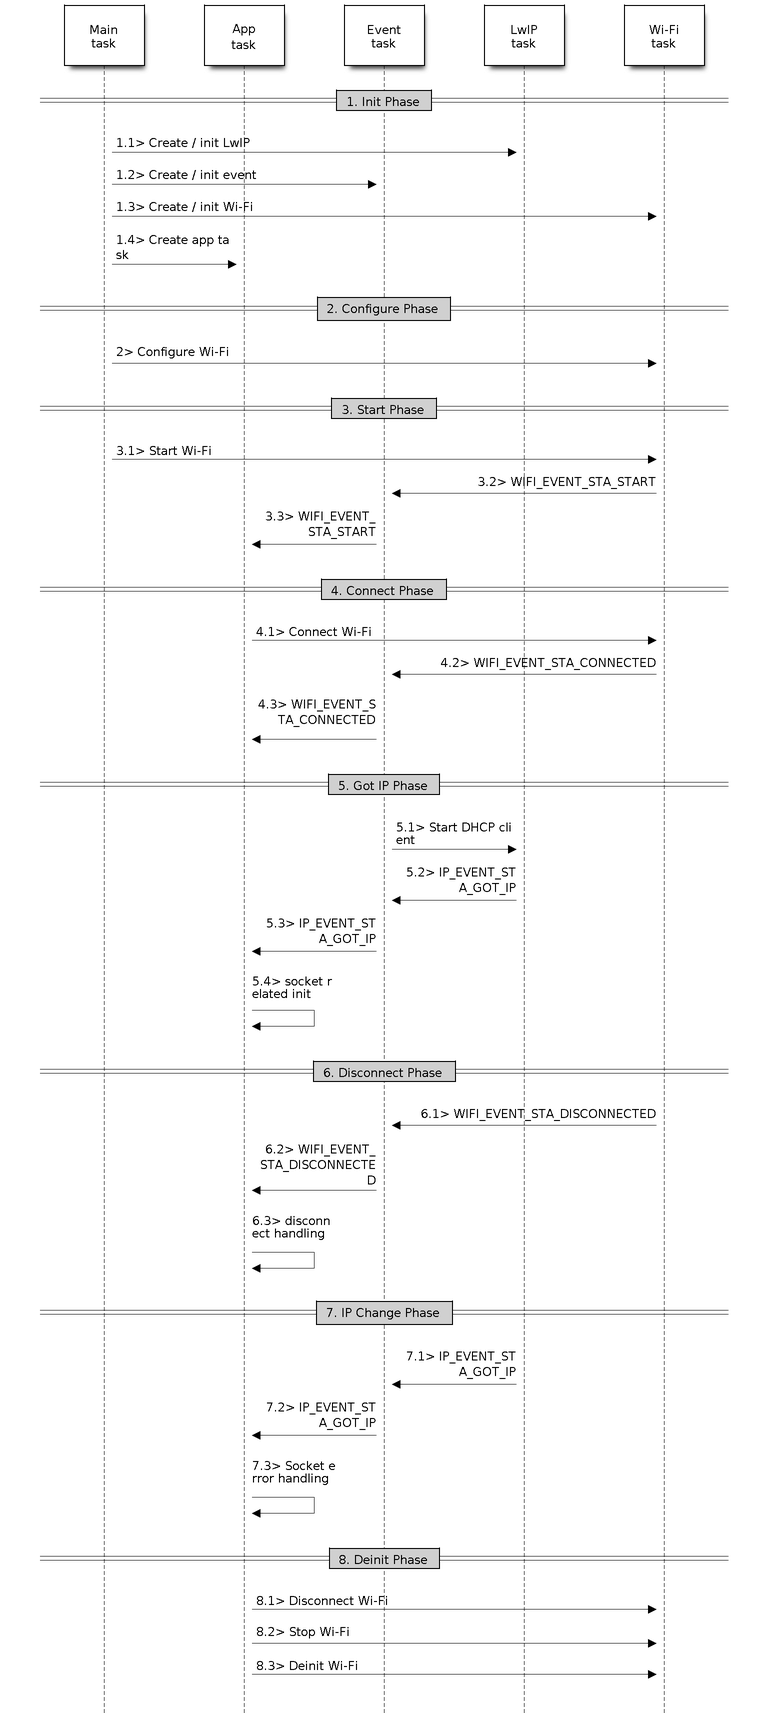
\includegraphics[width=\linewidth]{imgs/station_scenario}
		\caption{Primjer scenarija Wi-Fi povezivanja u načinu rada stanice \cite{espressif}}
		\label{fig:station_scenario}
	\end{minipage}
	\hspace*{\fill}
	\begin{minipage}[t]{0.4\textwidth}
		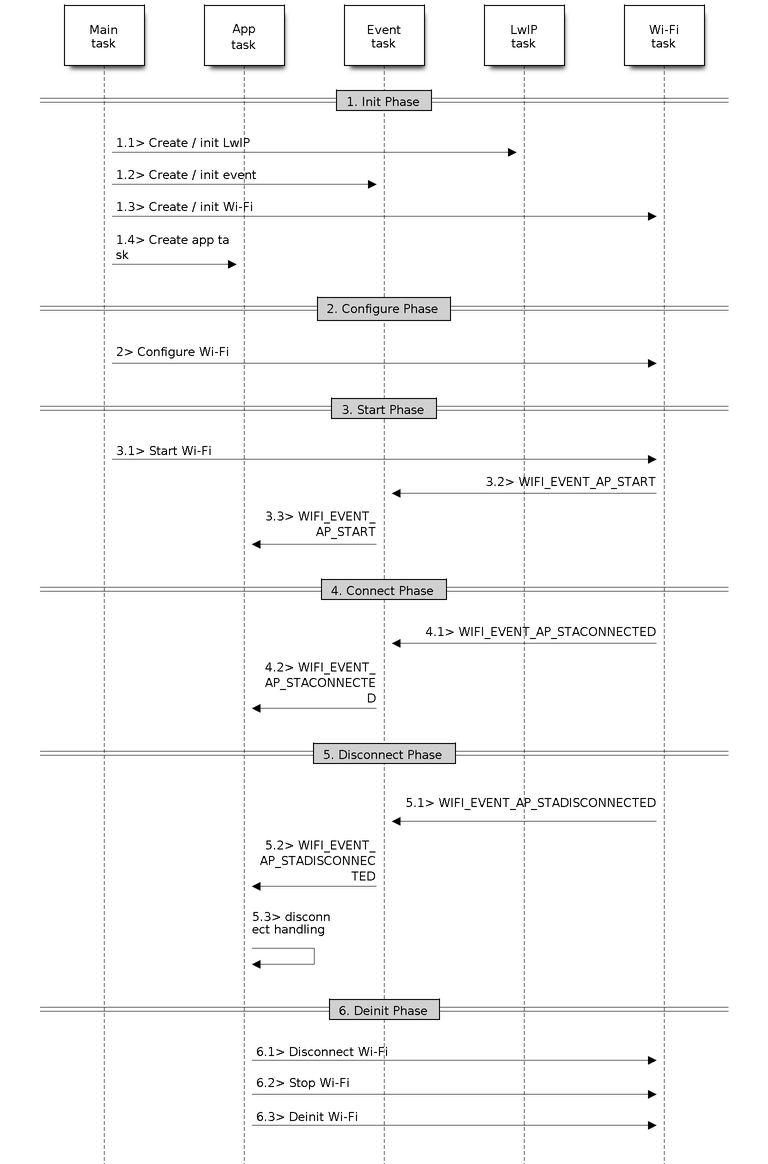
\includegraphics[width=\linewidth]{imgs/ap_scenario}
		\caption{Primjer scenarija Wi-Fi povezivanja u načinu rada pristupne točke \cite{espressif}}
		\label{fig:ap_scenario}
	\end{minipage}
\end{figure}

U modulu ESP32 stavljen je veliki naglasak na mehanizme uštede energije, što se također preslikava na korištenje Wi-Fi veze. Modul pruža načine uštede energije i pri radu kao stanica i pristupna točka, no neke značajke nisu podržane u pristupnoj točki. Modul pri neaktivnosti može otići u stanje mirovanja (engl. \textit{sleep mode}). Postoje dva načina uštede energije u načinu rada stanice: minimalna i maksimalna ušteda. Pri minimalnoj uštedi stanica se budi iz stanja mirovanja nakon svakog DTIM intervala (engl. \textit{Delivery Traffic Indication Message}). Ovim se načinom ne gube globalno emitirane poruke (engl. \textit{broadcast}) jer se one prenose nakon DTIM intervala. Međutim, ova metoda ne štedi puno energije ako je pristupna točka na koju je spojen modul postavila malen interval. Pri maksimalnoj uštedi moguće je znatno produžiti vrijeme mirovanja u odnosu na DTIM interval, no ovime se riskira gubitak globalno emitiranih poruka. 

\section{BLE protokol}

BLE je vrsta bežične komunikacije namijenjena komunikaciji kratkog dometa s niskom potrošnjom energije. Razvijen je kako bi se postigao standard vrlo male snage koji radi s baterijom veličine kovanice (engl. \textit{coin-cell batteries}) nekoliko godina. U odnosu na proizvode koji koriste klasičnu Bluetooth tehnologiju, BLE uređaji troše samo dio energije te omogućavaju malenim uređajima s malim baterijama bežično povezivanje s uređajima koji koriste Bluetooth. BLE protokol ostvaruje nisku potrošnju tako što boravi u stanju mirovanja dok nije povezan s drugim uređajima. Zbog toga može prenositi male količine podataka u kratkom vremenskom periodu. \cite{blevsbluetooth}

BLE radi u istom opsegu od 2,4 GHz kao i standardni Bluetooth, no koristi različite kanale od standardnog Bluetootha. Koristi 40 kanala od 2 MHz za prijenos podataka korištenjem modulacije Gaussova pomaka frekvencije (metoda koja se koristi za glatkije prijelaze između podatkovnih impulsa), zbog čega skokovi frekvencije proizvode manje smetnji u usporedbi sa standardnom Bluetooth komunikacijom.

BLE je tehnologija adaptivnog skakanja frekvencije (engl. \textit{Adaptive frequency hopping} - AFH) koja može koristiti samo podskup svih dostupnih frekvencija kako bi se izbjegle sve frekvencije koje koriste druge neprilagodljive tehnologije. To omogućuje prelazak s lošeg kanala na poznati dobar kanal korištenjem specifičnog algoritma za skakanje frekvencije, koji određuje sljedeći dobar kanal za korištenje. 

Arhitektura BLE tehnologije naziva se još i BLE stog zbog slojevite strukture. Stog se sastoji od dvije glavne komponente: BLE upravljač (engl. \textit{controller}), koji prenosi podatke, te BLE domaćin (engl. \textit{host}), koji definira odnos povezanih uređaja. Prikaz arhitekture stoga nalazi se na slici \ref{fig:ble_stack}.

\begin{figure}[ht]
	\centering
	\includegraphics[scale=0.8]{imgs/ble\_stack}
	\caption{Arhitektura BLE stoga \cite{espressif}}
	\label{fig:ble_stack}
\end{figure}

Osnovni profil koji implementiraju svi Bluetooth uređaji naziva se generički profil pristupa (GAP), koji pruža puni standardni okvir za kontrolu BLE uređaja u komunikacijskim metodama od točke do točke (engl. \textit{point-to-point}) i emitiranju podataka. Profil definira kako BLE uređaji mogu otkriti druge uređaje i povezati se s njima te kako uspostaviti sigurnost i privatnost preko veze. Također detaljno opisuje na koji način uređaji mogu biti odašiljači i promatrači te prenositi podatke bez da su u stanju veze, odnosno bez direktne povezanosti s drugim uređajem. Postoje četiri uloge GAP profila:

\begin{itemize}
	\item emiter (engl. \textit{broadcaster}): šalje oglase,
	\item promatrač (engl. \textit{observer}): prima oglase,
	\item periferija (engl. \textit{peripheral}): uvijek u načinu oglašavanja i u ulozi \textit{slave}, 
	\item centar (engl. \textit{central}): nikada ne šalje oglase, uvijek u \textit ulozi {master}.
\end{itemize}

Generički atributni profil (GATT) odgovoran je za razmjenu podataka i određuje njihovu strukturu. Definira dvije uloge uređaja: GATT poslužitelj i GATT klijent. BLE uređaj može implementirati samo jednu, ili pak istovremeno obje uloge.

GATT poslužitelj najčešće je implementiran u ugradbenom računalu. Poslužitelj implementira tablicu atributa (adresirani dijelovi informacija) strukturiranu u obliku usluga i karakteristika; točnije, sadrži korisne podatke kojima može pristupiti udaljeni klijent. Usluge su skupine karakteristika, odnosno korisničkih podataka koje uređaj želi poslati. Na slici \ref{fig:ble_profile_char} prikazana je opisana hijerarhijska struktura podatkovnog paketa. 

\begin{figure}[ht]
	\centering
	\includegraphics[scale=0.4]{imgs/ble\_profile\_char}
	\caption{Struktura paketa koji se šalju BLE protokolom \cite{ble_profile_char}}
	\label{fig:ble_profile_char}
\end{figure}


BLE protokol nudi tri komunikacijske mogućnosti različitih topologija veze. Prikazane su na slici \ref{fig:ble_com_options}. 

\begin{figure}[ht]
	\centering
	\includegraphics[scale=0.4]{imgs/ble\_com\_options}
	\caption{Komunikacijske mogućnosti u BLE-u \cite{ble_profiles}}
	\label{fig:ble_com_options}
\end{figure}

Prva i najraširenija metoda jest od točke do točke (engl. \textit{point-to-point}). Koristi se u uređajima gdje je povezivanje 1:1, odnosno gdje je moguće međusobno spajanje samo dva uređaja. Većina uređaja u svakodnevnoj uporabi koriste ovu topologiju, primjerice zvučnici, pametne igračke, satovi i uređaji za praćenje zdravlja. Također se naziva i komunikacijom usmjerenom na povezivanje (engl. \textit{connection-oriented communication}), budući da se temelji na povezivanju dvaju uređaja. Iako početna verzija ove metode dopušta spajanje samo dva uređaja, nove verzije protokola omogućuju vezu n:1, što omogućava spajanje više uređaja na jedan centralni uređaj. Razlikuje se od metode emitiranja podataka zbog uloge čvorova u spoju. BLE stog podržava sigurnosnu zaštitu za ovu vrstu topologije 128-bitnim AES algoritmom, no ovom je metodom spajanja zaštita opcionalna. 

U ovom načinu povezivanja uređaji implementiraju jednu od dvije uloge GAP profila, a to su centar i periferija. Centralni je uređaj najčešće onaj koji troši više resursa, primjerice računalo ili mobitel, dok je periferni uređaj ugradbeno računalo s niskom potrošnjom. Nove verzije protokola podržavaju spajanje više perifernih uređaja na centralni.

Iduća metoda je emitiranje podataka (engl. \textit{data broadcast}), čija je topologija povezivanja 1:n. Emitiranje podataka naziva se još i komunikacijom bez povezivanja. Ovo je jednosmjerna metoda komunikacije gdje uređaj emitira svoje podatke svim susjednim uređajima u RF rasponu. Također se koristi za usluge lokacije niske točnosti (margina pogreške od 1,5 metra), primjerice osnovna navigacija u zatvorenom prostoru i pronalaženje puta. Centralni čvor koji emitira podatke još se naziva i BLE odašiljačem. Arhitektura BLE protokola ne podržava sigurnost ovakve vrste povezivanja, no sigurnosni algoritmi se po potrebi mogu implementirati u aplikacijskom sloju. 

Ovaj način povezivanja podržava uloge emitera i promatrača. Pri emitiranju podataka, središnji čvor odnosno odašiljač isporučuje podatke jednosmjernom vezom. Šalje reklamne pakete s podacima u ulozi oglašivača, dok promatrači skeniraju reklamne pakete i tako primaju podatke. Konfiguracija emitiranja podataka najprikladnija je za senzore koji otvoreno emitiraju svoje javne podatke svim zainteresiranim susjednim uređajima. Reklamni se paketi mogu konfigurirati tako da pri njihovu skeniranju promatrač, po potrebi, može zatražiti dodatne informacije od odašiljača posebnim zahtjevom. Paket zahtjeva za skeniranje ne može sadržavati nikakve korisničke podatke.

Postoji nekoliko nedostataka ovakve vrste povezivanja. Ova topologija podržava isključivo jednosmjernu vezu, što znači da odašiljač ne može primiti nikakvu korisnu informaciju od promatrača. Isto tako, svi uređaji u blizini primaju odašiljane pakete, te nije moguće slati podatke samo jednom uređaju. 

Posljednji način jest mrežna topologija (engl. \textit{mesh}). BLE \textit{Mesh} koristi se za uspostavljanje komunikacije više-prema-više uređaja (n:n). Omogućuje stvaranje složenih velikih mreža i idealan je za nadzor, kontrolu i sustave automatizacije gdje je potrebna pouzdana međusobna komunikacija mnoštva uređaja. Ova metoda povećava domet i pokrivenost izvan BLE RF dometa, te pomaže u izbjegavanju fizičkih prepreka. Sigurnost je obavezna u ovom načinu rada, te je podržana BLE stogom. \cite{ble_profiles}


\eject